% !TEX root=/home/tavant/these/manuscript/src/manuscript.tex
\FloatBarrier
\section{Comparison of the \acs{DR} with the \acs{PIC} simulations}
  \label{sec-DR-results}
  
  

  \subsection{Temporal evolution of the distribution functions in the \acs{PIC} simulation} \label{subsec-VDFpic}
  
  To beging with, we visualize and comment the distribution functions measured in the \ac{PIC} simulation.
  \Cref{fig-vdfs_pic_time} shows at different moments in the simulation the ion and electron azimuthal velocity distribution functions, normalized.
  The velocities are normalized by the thermal speed of the respective species.
  To guide the reading of the figure, is added the  theoretical electron drift velocity $u_e = \frac{E_z}{B_r}$, normalized to the electron thermal speed, as well as the ion sound speed $c_s$, normalized to the ion thermal velocity.
  The distributions are averaged in time over $4\,\nano\second$, and in space over all the azimuthal direction.
  In the radial direction, the distributions are averaged over a small length at the center of the channel, between $r=0.45\,\centi\meter$ and $r=0.55\,\centi\meter$.
  
  \begin{figure}[!hbt]
    \centering
    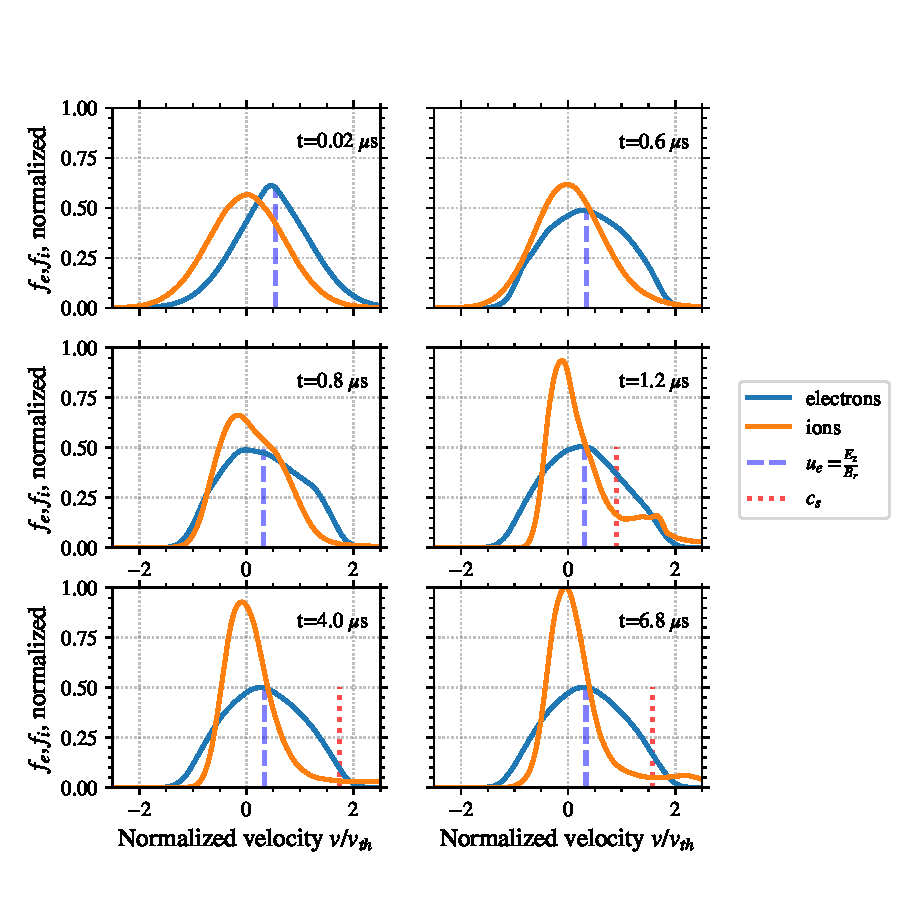
\includegraphics[width=0.95\textwidth]{Distributions_time_evolution_2.pdf}
    \caption{Electron and ion normalized azimuthal velocity distribution functions. The velocity in abscissa is normalized by the thermal speed of the corresponding species. Is overlaid the theoretical $E\times B$ drift velocity of the electrons $u_e = \frac{E_z}{B_r}$, and the ion sound speed $c_s$ normalized by the ion thermal velocity.}
    \label{fig-vdfs_pic_time}
  \end{figure}
  
  We can observe in \cref{fig-vdfs_pic_time} that the electron mean velocity is always the $E \times B$ drift velocity, which is of the order of one quarter of the electron thermal speed.
  On the other hand, at the beginning of the simulation the mean velocity of the ion is null.
  But we can see that starting from $t=.8\,\micro\second$, the ions are dragged in the same direction that the electron drift.
  This is characteristic of the ion-wave trapping \citep{lafleur2017a}
  Here, we have to be careful not to misread the figure.
  As we have $v_{th, e} > v_{th, i}$, the effective drift velocity of the ion is much less that the electron.
  % \inlinenote{Give the values here, like $ u_e, c_s, v_th$, etc. \\ Anne: oui pour mettre des valeurs}
  
  We can see that a small population of high energy ions is generated, because of particle-wave interactions.
  This leads to both an increase ion temperature, and the formation of a drift velocity in the azimuthal direction.
  The high energy ion population comes from ion trapping, as we can see that their velocity is of the order of the ion sound speed, which is close to the wave phase velocity \citep{lafleur2018}.
  
  As both electron and ion velocity distribution functions are far from a drifting Maxwellian, we will study the influence of both distributions in the calculations of the dispersion relation.
  
  
  % \FloatBarrier
  \subsection{Resolution of the electron cyclotron drift instability} \label{subsec-ECDIPIC}
  
  
    As observed in \Cref{sec-PIC-ECDI}, the simulation begins by a linear growth of the instability.
    Previous results obtained with \LPPic \citep{croes2017a} showed no resonances during this period.
    However, these results where obtained with Lafleur's convection model, as introduced in \cref{sec-reinjectionnoise}.
    Here, the results where obtained with the modified model, inducing less noise.
    The parameters used for the simulation are given in \cref{tab-evdfpicparams}.
    
    We can see in \Cref{fig-phi_fluctuation_summary}  a snapshot of the plasma potential fluctuation in the azimuthal direction \[ \delta \phi(r, \theta) = \phi(r, \theta) - < \phi(r, \theta) >_{ \theta}, \]
    at four different times during the growth of the instability.
    For these results, we increased the azimuthal length $L_{\theta}$ from $2.5$ to $6.2\,\milli\meter$ compared to the simulations of \cref{ch-2,sec-PIC-ECDI}, so that the instability characteristics, as the wavenumber $k$, are more distinguishable.
    We observe no significant differences on the simulation results.
    However, the simulation time is doubled in this case, so only the first microseconds have been simulated.
    

    
    \begin{figure}[!hbt]
      \centering
      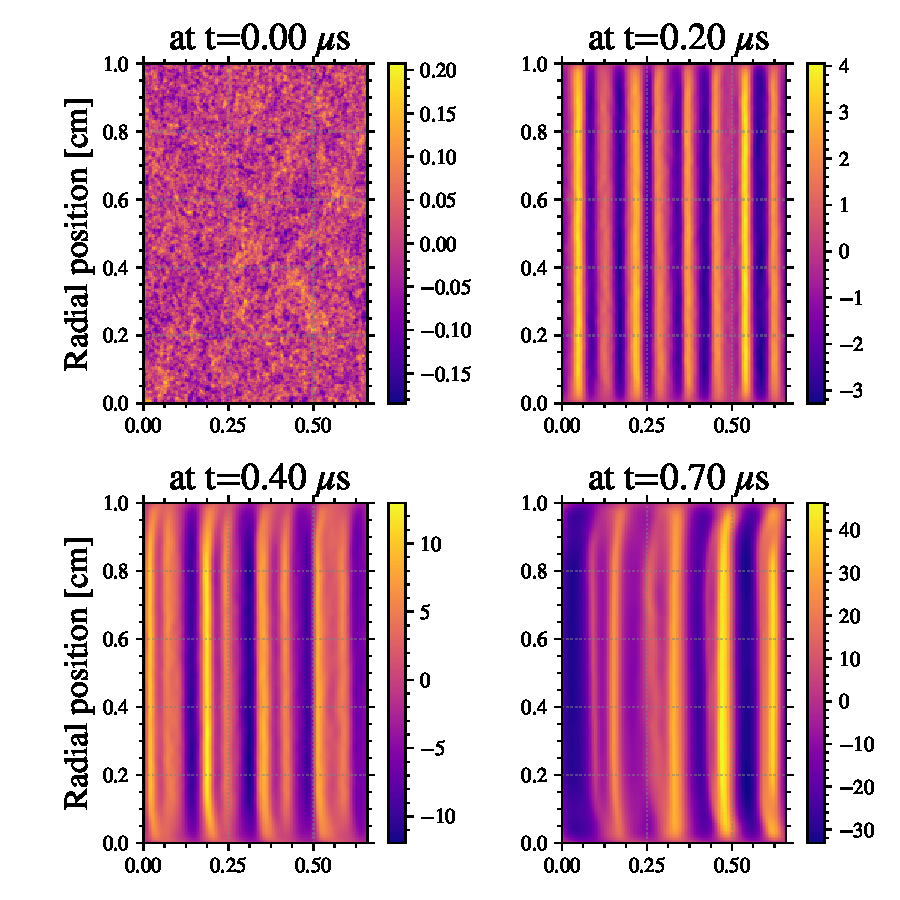
\includegraphics[width=0.8\textwidth]{phi_fluctuation_summary.pdf}
      \caption{Snapshot of the plasma potential at different times during the linear phase of the simulation. The frequency spectra of each snapshot is showen in \cref{fig-phi_fluctuation_summary_FFT}. }
      \label{fig-phi_fluctuation_summary}
    \end{figure}
    
    At the beginning, we see fluctuations that can be due to both thermal fluctuation \citep{salpeter1960} or numerical noise due to particle discretization.
    Then, the instability rises.
    We can see that it starts with small wavelength ($\lambda \simeq 0.75\,\milli\meter$ at $t=0.2\,\micro\second$).
    After a short period, the short wavelength waves merges to form longer wavelength waves  ($\lambda \simeq 1.5\,\milli\meter$ at $t=0.7\,\micro\second$).
    
    
    \begin{figure}[!hbt]
      \centering
      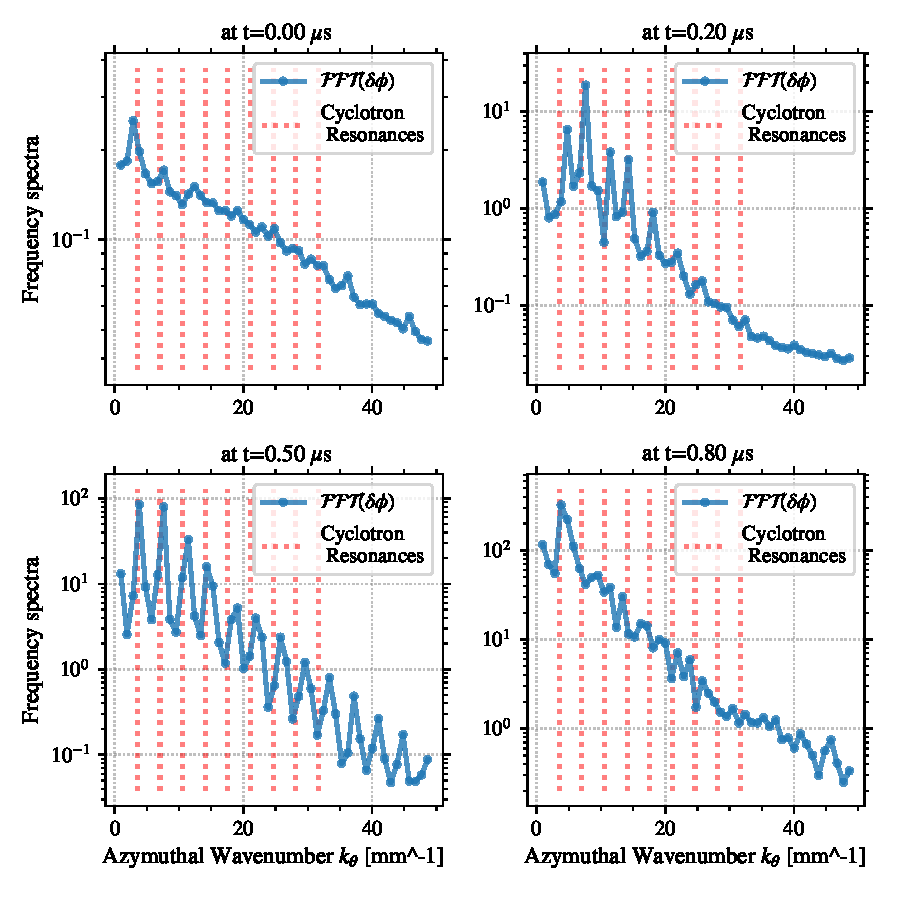
\includegraphics[width=0.8\textwidth]{phi_fluctuation_summary_FFT.pdf}
      \caption{Frequency spectra on the azimuthal instability presented in \cref{fig-phi_fluctuation_summary}. Each spectrum is averaged in the radial direction. The red dotted lines represent the cyclotron resonances.}
      \label{fig-phi_fluctuation_summary_FFT}
    \end{figure}
    
    This is also clearly seen on the frequency spectra, showed in \Cref{fig-phi_fluctuation_summary_FFT}.
    We can see in the spectra the resonances at the cyclotron wavenumber $k_0 = \frac{\oce}{u_e} \simeq 3.5\,\milli\meter^{-1}$.
    At $t=0.2\,\micro\second$, the most dominant mode is the second resonance, but the other resonances start to appear.
    At $t=0.4\,\micro\second$, all of the resonances are distinguishable, but their amplitude is strictly decreasing.
    Then, at $t=0.7\,\micro\second$, we can no longer see the resonances, except for the first one.
    As we observed during the first stages of the simulation the resonances in the Fourier spectrum, we solve the dispersion relation for the \ac{ECDI}.
    
    \vspace{1em}
    We solve the \ac{ECDI} dispersion relation of \cref{eq-drECDI} for $t=0.2, 0.4$ and $0.7\micro\second$ using both the Maxwellian hypothesis for the ions and electrons, and the velocity distribution functions measured in the \ac{PIC} simulations.
    The radial wavenumber taken is $k_r = 2 \pi/L_R \sim 0.6 \per\milli\meter$ \citep{lafleur2016,janhunen2018}.
    This value corresponds to $k_r \lde = 0.036$ at $t=0.2\,\micro\second$ and $k_r \lde = 0.044$ at $t=0.7\,\micro\second$, as the electron temperature increases.
    
    \begin{figure}[!hbt]
      \centering
      % \begin{tabular}{c}
        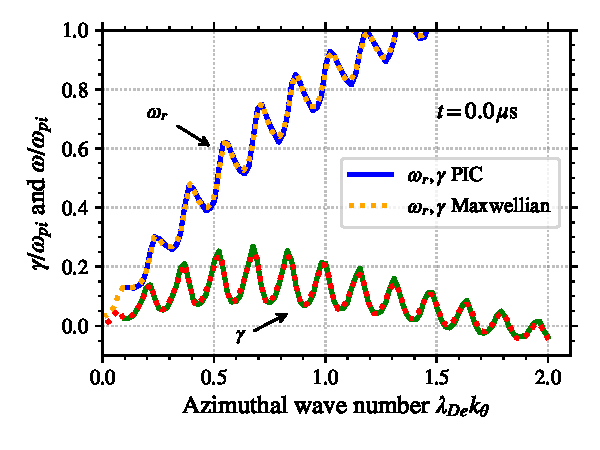
\includegraphics[width=0.49\textwidth]{ECDI_PIC_ionvcorrected_2mus.pdf} 
        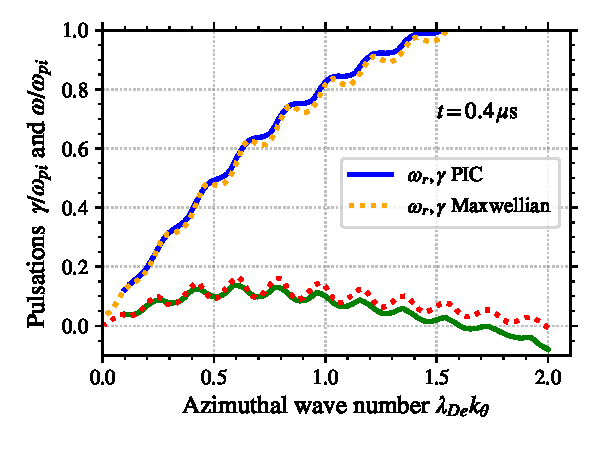
\includegraphics[width=0.49\textwidth]{ECDI_PIC_ionvcorrected_4mus.pdf} 
        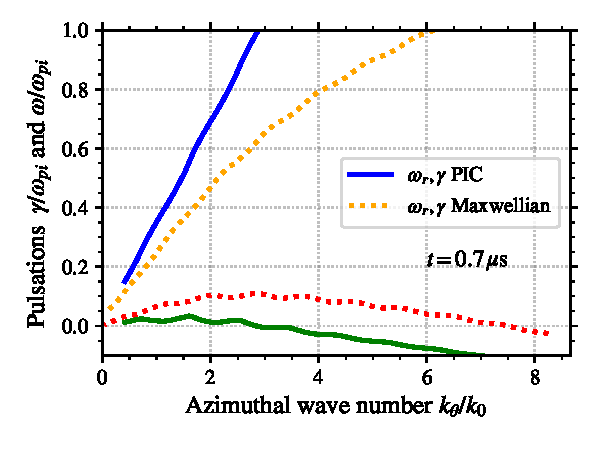
\includegraphics[width=0.49\textwidth]{ECDI_PIC_ionvcorrected_7mus.pdf} 
      % \end{tabular}
      \caption{Dispersion relation for the \acs{ECDI} using both (dotted lines) the Maxwellian hypothesis for the ions and electrons, and (solid lines) the velocity distribution functions measured in the \acs{PIC} simulations. The abscissa is normalized by the cyclotron resonance wavelength.}
      \label{fig-DRECDI}
    \end{figure}
    
    We can see in \Cref{fig-DRECDI} that the dispersion relation shows the cyclotron resonance at the beginning.
    However, the most growing wavelength is not the second harmonic, but the forth.
    After $t=0.4\,\micro\second$, the resonances broaden, and disappear.
    This is due to the increases of the radial wavelength used with respect to the Debye length $\lde$ \citep{lafleur2016a,ducrocq2006,cavalier2013}.
    The value of radial wavelength is discuss later in \cref{sec-DR-BC}.
    
    We can also observe that the deviation of the distribution function from the Maxwellian decreases the growth rate.
    This has been observed  in an axial-azimuthal \ac{PIC} simulation by \citet{lafleur2018}.
    This confirms that the exact distribution function should be used in the calculation of the dispersion relation, especially to determine the growth rate.
    \Cref{fig-DR_and_fft} shows a comparison of the \ac{2D} \ac{FFT} of the azimuthal electric field FFT$(E_{\theta})$ computed between  $t=0.6\,\micro\second$ and $t=1.2\,\micro\second$  with the three dispersion relations\string:
    \begin{itemize}
      \item the \ac{ECDI} general \ac{DR} obtained with the \ac{PIC} \ac{EVDF} at $t=0.6\,\micro\second$,
      \item the \ac{ECDI} \ac{DR} obtained with the Maxwellian hypothesis,
      \item the \ac{IAW} \ac{DR} using the analytic expression \cref{eq-MIAW}. 
    \end{itemize}
    The two first \ac{DR} are already showed in \cref{fig-DRECDI} with there corresponding growth rates.

    \begin{figure}[!hbt]
      \centering
      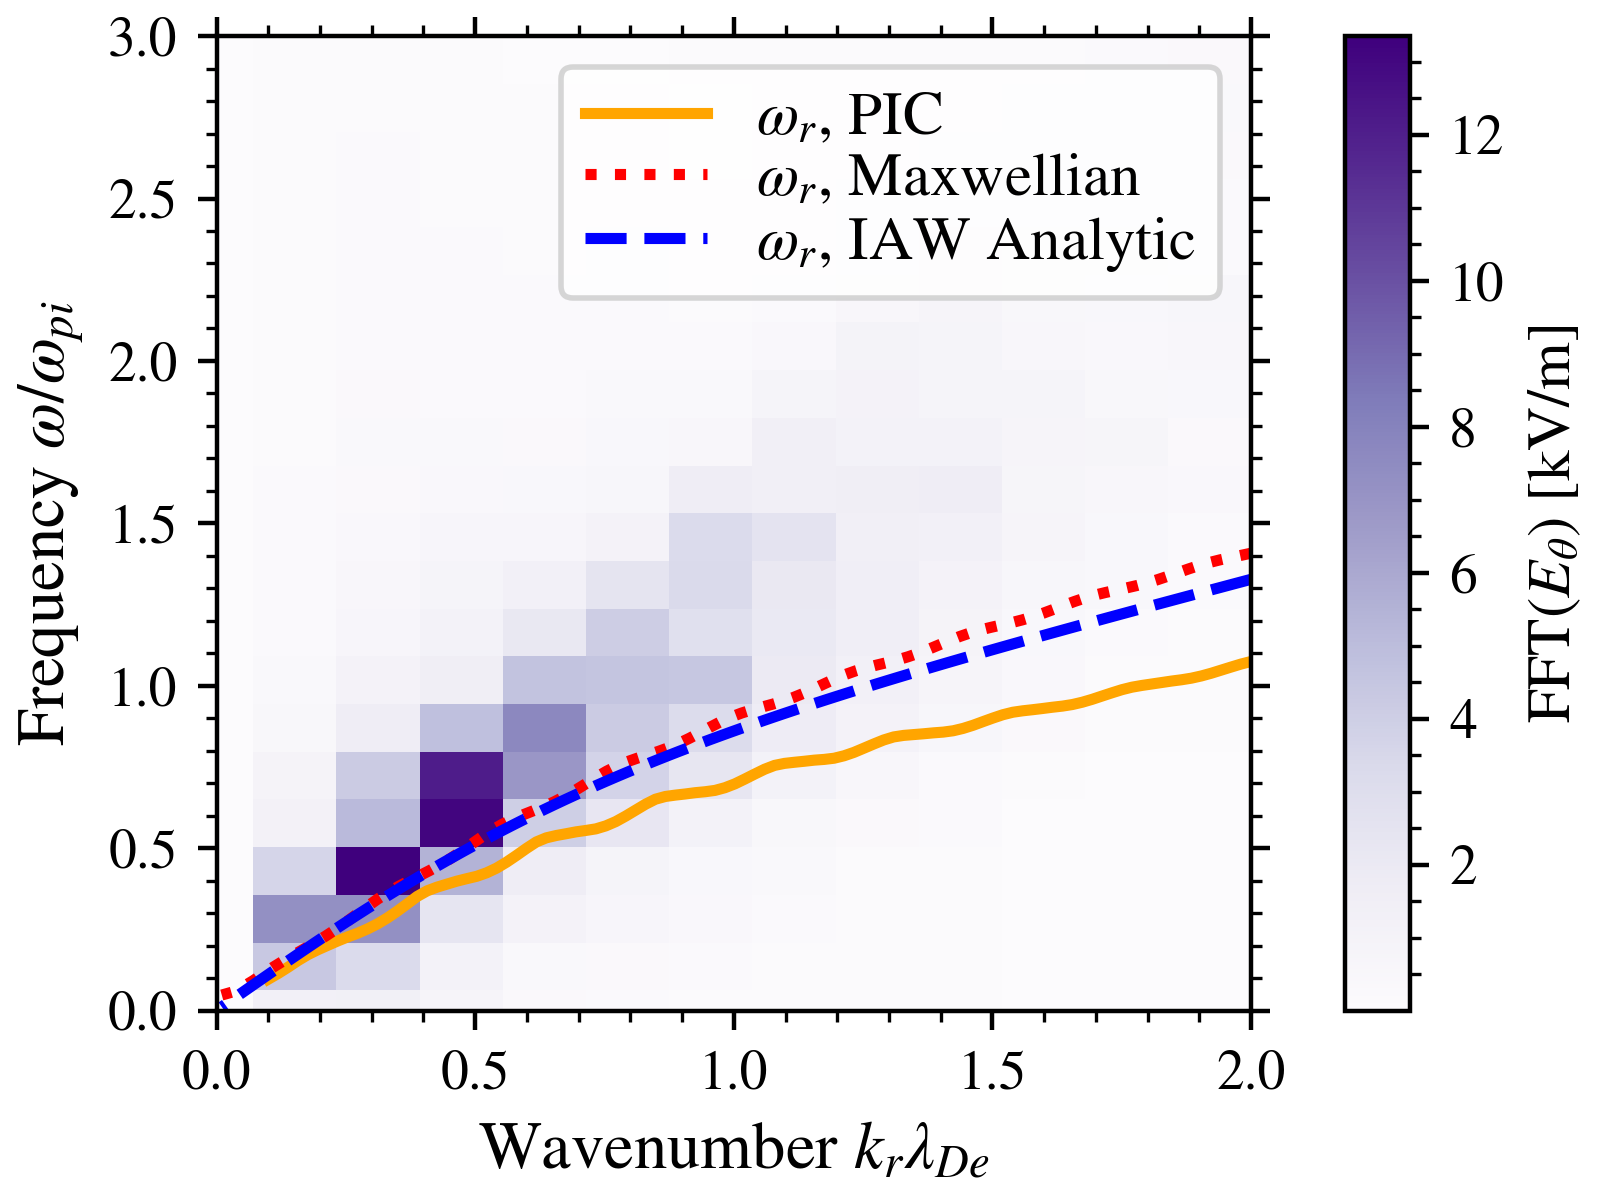
\includegraphics[width=\defaultwidth]{compe_fft_theo}
      \caption{Comparison of the \acs{2D} \acs{FFT} of the azimuthal electric field FFT$(E_{\theta})$ with the following \acs{DR}\string: (orange solid) \acs{ECDI} general \acs{DR} obtained with the \acs{PIC} \acs{EVDF}; (dotted red) \acs{ECDI} \acs{DR} obtained with the Maxwellian hypothesis; and (dotted blue) \acs{IAW} \acs{DR} using the analytic expression \cref{eq-MIAW}.   }
      \label{fig-DR_and_fft}
    \end{figure}
    
    From \Cref{fig-DR_and_fft}, we can see that the \ac{PIC} result does follow the \ac{ECDI} \ac{DR} with a very good correspondence.
    However, the differences between the three \ac{DR} are not significant, compared to the resolution of the \ac{2D} \ac{FFT}.
    On top of that, the \ac{IAW} \ac{DR} returns almost the same values than the \ac{ECDI} \ac{DR}, as the resonances are no more present.
    
  \FloatBarrier
  \subsection{Resolution of the ion acoustic wave dispersion relation} \label{subsec-VDFIAW}
  
  We have seen in the previous \cref{subsec-ECDIPIC} that the full \ac{ECDI} dispersion relation is not needed, but can instead be approximated by the \ac{IAW} \citep{lafleur2018,janhunen2018,taccogna2019}.
  The \ac{IAW} relation can be solved with several hypotheses (see \cref{sec-geneDR} for more details)
  \begin{enumerate}
    \item Simplified analytical values,
    \item Maxwellian electrons, cold ion ($\Ti = 0\,\volt$),
    \item Maxwellian electrons and ions ($\Ti > 0\,\volt$),
    \item Non-Maxwellian electrons, Maxwellian ions ($\Ti > 0\,\volt$),
    \item Non-Maxwellian electrons and ions.
  \end{enumerate}
  
  We will use all of these cases, and compare them to the \ac{PIC} simulation results.
  We want to obtain the temporal evolution of the solution.
  In practice, we will only follow the evolution of the most growing wave.
  In order to find the most growing wave, we solve the dispersion relation for different values of $k$.
  Over all of the solutions obtained, we select the one corresponding to the maximum value of $\gamma$.
  We use 100 values between $k=0.02 \lde$ and $k = 2 \lde$.
  \Cref{fig-Example_of_DR_IAW} illustrates the protocol used for 3 different cases.
  We can see the maximum of the growing rate, and its frequency.
  
  \begin{figure}[hbt]
    \centering
    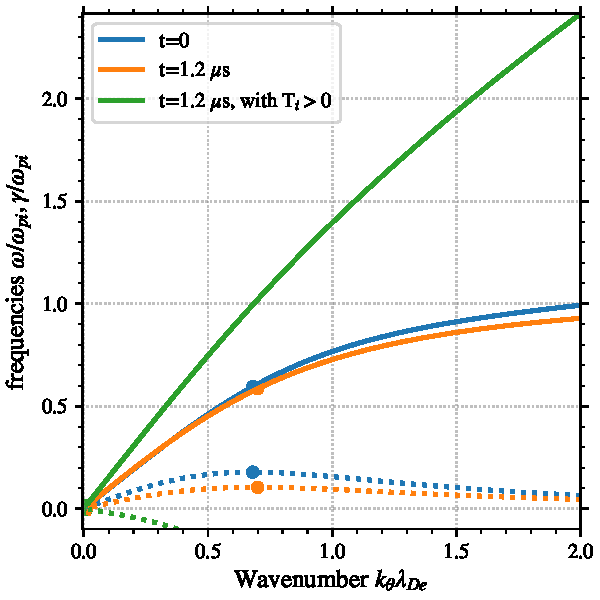
\includegraphics[width=4.5in]{Example_of_DR_IAW.pdf}
    \caption{Illustration of the \acs{IAW} dispersion relation obtained at two different time ($t=0$ and $t=1.2\,\micro\second$), (solid line) the wave frequency $\omega$, and (dotted line) the growth rate $\gamma$, using the hypothesis of Maxwellian distribution functions for both electrons and ions. The electron temperature measured in the simulation is always used, but the ion temperature is only used once. The most growing solution is marked with a circle on the growing rate and the frequency.}
    \label{fig-Example_of_DR_IAW}
  \end{figure}
  
  
  This calculation is automated for the whole duration of the simulation.
  The velocity distribution functions, when used, are obtained from the \ac{PIC} simulation the same way that in \cref{subsec-VDFpic}.
  \Cref{fig-time_wave} shows the temporal evolution of the three characteristics of the most growing wave: the growth rate $\gamma$, the azimuthal wavenumber $k$ and the frequency $\omega$.
  \begin{figure}[hbt]
    \centering
    % 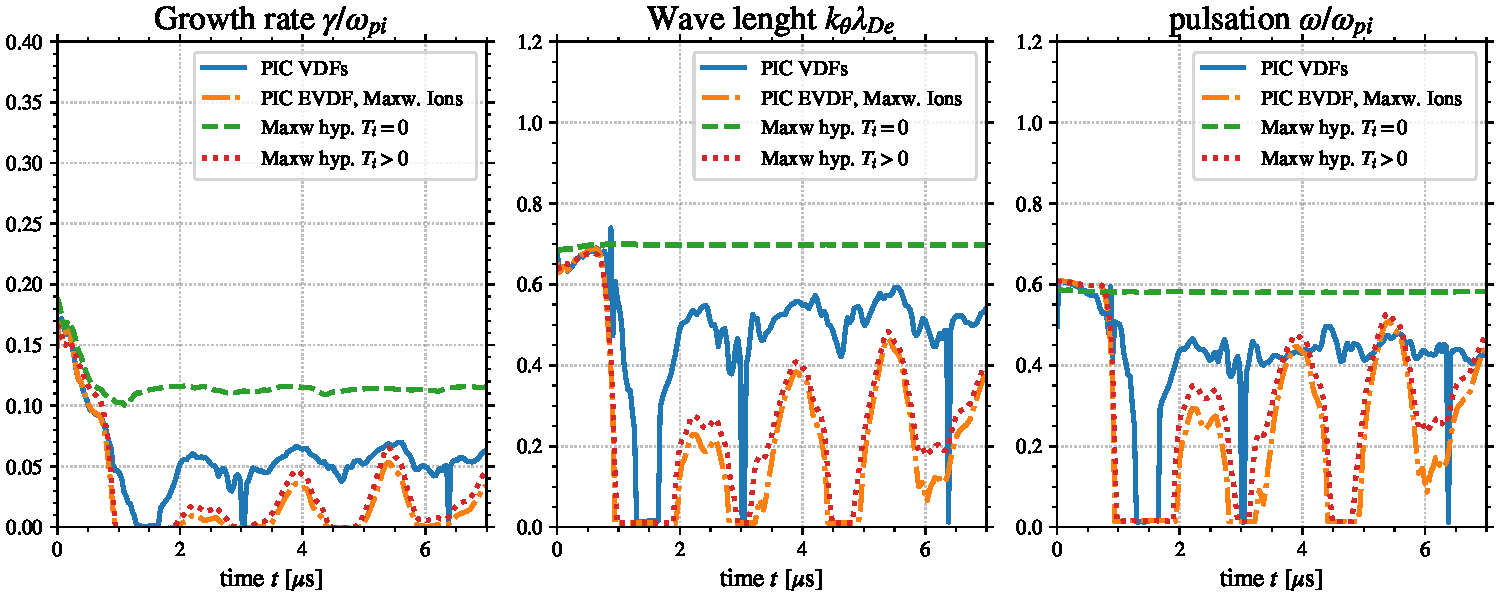
\includegraphics[width=\textwidth]{GrowthRate_time_evolution_250_ter.pdf}
    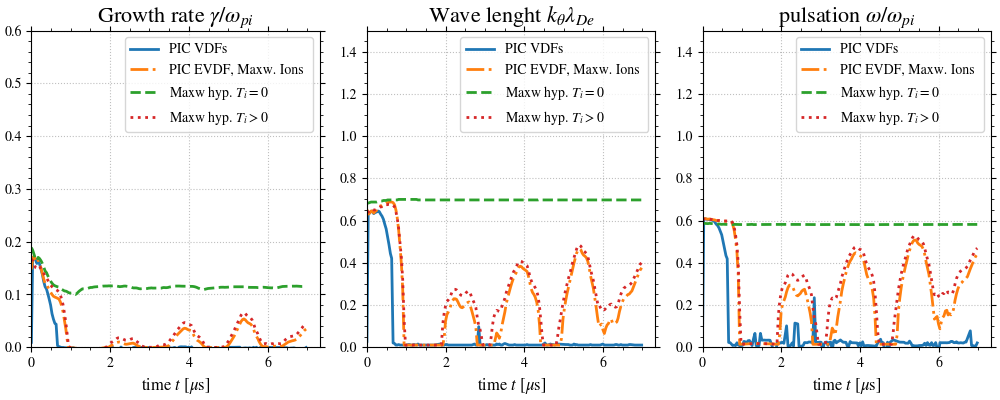
\includegraphics[width=\textwidth]{GrowthRate_time_evolution_250_again.png}  %inverted ion velocity as a correction, to look like Lefleur... :/
    \caption{Temporal evolution of the growth rate $\gamma$, the azimuthal wavenumber $k$ and the frequency $\omega$ for the most growing wave, obtained with several hypotheses on the dispersion relation. See text for more precisions. }
    \label{fig-time_wave}
  \end{figure}
  
  Three different behaviors are observed depending on the hypotheses used.
  First, the solution of the dispersion relation with Maxwellian electrons and cold ions (dashed green line in \cref{fig-time_wave}) presents a solution of $\omega$ and $k$ constant in time, and very close to the analytical values, beeing $k \lde = 1/\sqrt{2}$ and $\omega = \opi/\sqrt{3}$.
  However, it also presents a constant growth rate.
  Secondly, we observe that the solutions given with Maxwellian ions of temperature not zero are relatively similar for both the Maxwellian electrons  (dotted red line) and using the electron velocity distribution function measured in the \ac{PIC} simulation (dash-dotted orange line).
  In these cases, the growth rate decreases regularly to zero.
  
  Interestingly, the periods during which the growth rate is zero (firstly between $t=1\,\micro\second$ and $t=2\,\micro\second$, then around $t=3\,\micro\second$ and so on) correspond precisely to the periods during which the wave energy density decreases in \cref{fig-tempITcrit}.
  This means that the decrease of the wave amplitude would only be due to the ion temperature, and not its distribution function.
  However, we note that the value of the ion temperature $\Ti$ is highly affected by the population of ions trapped, as seen in \cref{subsec-VDFpic}.
  Hence, the effect of the trapped particle is indeed present, but only via its impact on the temperature.
  
  \vspace{1em}
  To finish with, we solved the \ac{IAW} dispersion relation without any hypothesis on the velocity distribution functions, by using the one measured in the PIC simulations (blue solid line in  \cref{fig-time_wave}).
  In this case, the beginning ($t < 1 \,\micro\second$) is quite similar to the other results.
  However, after that ($t > 1 \,\micro\second$) the growth rate never rises above zero, expect very slightly around $t=4\,\micro\second$.
  This result is non consistent with the observations of \cref{sec-PIC-ECDI}, where we saw that the instability amplitude is modulated over the whole simulation time.
  It is also in contrast with \citet{lafleur2018}, where the authors obtained a non-zero growth rate in an axial- azimuthal geometry.
  
  Up to now, there is non apparent explanation to the dependency  observed between the numerical resolution of the \ac{DR} and the results of the \ac{PIC} simulation.
  It could be due to an error in the numerical algorithm, on both on the theory and in the implementation.
  Concerning the theory, we have seen in \cref{sec-DR-solver} that the numerical algorithm used to compute the plasma dispersion function $\tilde{Z}$ proposed by \citet{xie2013} does not return a good result for certain argument complex values.
  In addition, the truncation of the number of Fourier bases at $N=64$, which works well with a Maxwellian distribution, could generate a significant error when using distribution function far from a Maxwellian.
  In our specific case, the ion population is composed of a majority of cold Maxwellian ions and a small number of high energetic trapped ions.
  It is possible that this kind of distribution function is not well taken into account by the current algorithm.
  
  Concerning the implementation of the algorithm, we tried to test and validate the code as much as we can, with systematic comparaisons to analytic values.
  But the presence of an error is always possible, that was not observed on the analytic functions.
  A common practice to validate a simulation code when no theoretical solution can be used to compare to is to use a Benchmark \citep{turner2013}.
  As a dispersion relation solver for general distributions would benefit the whole plasma physics community, developing such a benchmark that would compare the solution of independent implementations of the same algorithm, or different algorithm, seems very interesting.
  
  \FloatBarrier